\subsection{IU1 Iniciar sesión}

\subsubsection{Objetivo}
	Controlar el acceso al sistema mediante cuentas de usuario de manera que cada usuario acceda solo a las funciones habilitadas para su perfil.

\subsubsection{Diseño}
	Esta pantalla aparece al iniciar el sistema. Para ingresar al mismo se debe escribir el correo electrónico y password. 

\begin{figure}[htbp!]
		\centering
			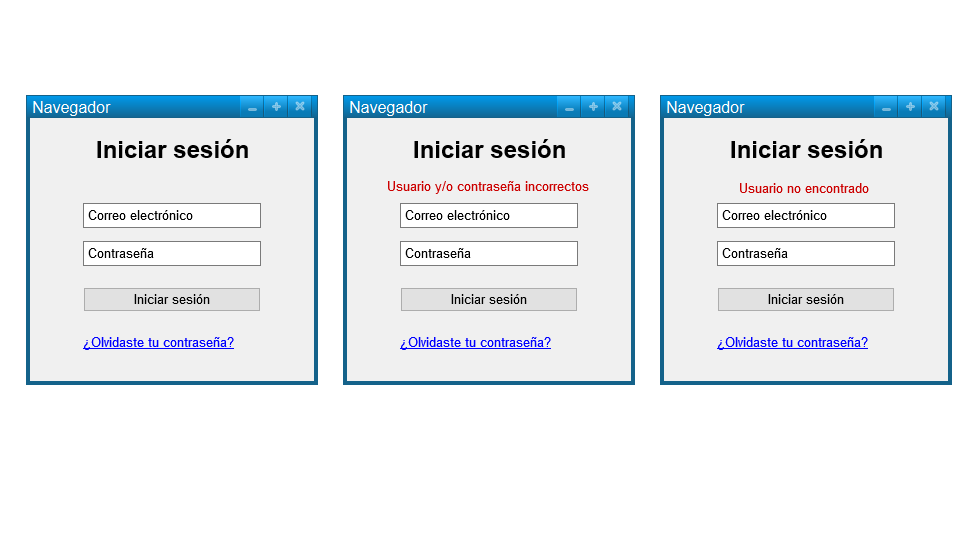
\includegraphics[width=0.8\textwidth]{images/UI1}
		\caption{UI1 Iniciar sesión}
	\end{figure}


\subsubsection{Salidas}
	Ninguna.

\subsubsection{Entradas}
Correo electrónico y contraseña del usuario.

\subsubsection{Comandos}
\begin{itemize}
	\item \IUbutton{Iniciar sesión}:  Verifica que el correo esté registrado en alguna cuenta y la contraseña ingresada corresponda con la contraseña registrada en la base de datos. Si la verificación es correcta muestra la \IUref{UI2}{Home}.	
\end{itemize}

\subsubsection{Mensajes}
	\begin{Citemize}
		\item {\bf MSG1a} Usuario y/o contraseña incorrectos.
        \item {\bf MSG1b} Usuario no encontrado.
	\end{Citemize}
    
    
%---------------------------------------------------------------------------------
\subsection{IU3 Registrar paciente}

\subsubsection{Objetivo}
	Realizar el registro del paciente con los datos requeridos para que dicho paciente pueda realizar una cita para consulta. 

\subsubsection{Diseño}
	Esta pantalla aparece al iniciar sesión como enfermera.

\begin{figure}[htbp!]
		\centering
			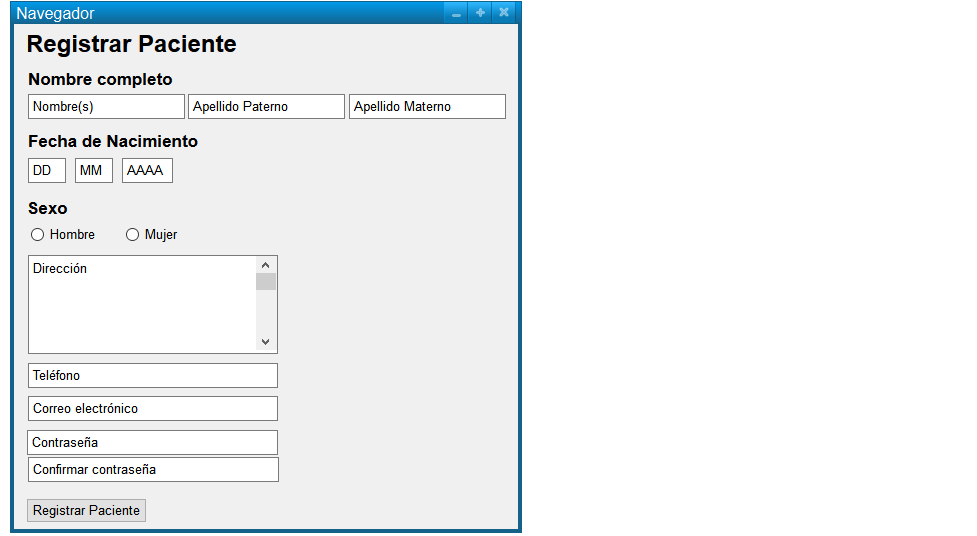
\includegraphics[width=0.8\textwidth]{images/UI3}
		\caption{UI3 Pantalla registrar paciente}
	\end{figure}


\subsubsection{Entradas}
\begin{itemize}
\item Nombres, apellido paterno y apellido materno del paciente.
\item Fecha de nacimiento (DD/MM/AAAA).
\item Sexo del paciente (Hombre o Mujer).
\item Dirección del paciente.
\item Teléfono.
\item Correo electrónico.
\item Contraseña y confirmación de contraseña.

\end{itemize}

\subsubsection{Comandos}
\begin{itemize}
	\item \IUbutton{Registrar paciente}:  Verifica que los datos sean correctos. Si la verificación es correcta muestra \IUref{UI2}{Home}.	
\end{itemize}

\subsubsection{Mensajes}
	\begin{Citemize}
		\item {\bf MSG3a} “Datos incorrectos”.
        \item {\bf MSG3b}  “Correo electrónico ya existente en la base de datos”.
	\end{Citemize}
    
    
    